\documentclass[9pt,a4paper,]{extarticle}

\usepackage{f1000_styles}

\usepackage[pdfborder={0 0 0}]{hyperref}

\usepackage[numbers]{natbib}
\bibliographystyle{unsrtnat}


%% maxwidth is the original width if it is less than linewidth
%% otherwise use linewidth (to make sure the graphics do not exceed the margin)
\makeatletter
\def\maxwidth{ %
  \ifdim\Gin@nat@width>\linewidth
    \linewidth
  \else
    \Gin@nat@width
  \fi
}
\makeatother


% disable code chunks background
%\renewenvironment{Shaded}{}{}

% disable section numbers
\setcounter{secnumdepth}{0}

%% added by MLS, this is not in the F1000 style by default %%

\hypersetup{unicode=true,
            pdftitle={BASiCS workflow: a step-by-step analysis of expression variability using single cell RNA sequencing data},
            pdfkeywords={Single-cell RNA sequencing, expression variability, transcriptional noise, differential expression testing},
            colorlinks=true,
            linkcolor=Maroon,
            citecolor=Blue,
            urlcolor=Orange,
            breaklinks=true}

%% End added by MLS %%

\setlength{\parindent}{0pt}
\setlength{\parskip}{6pt plus 2pt minus 1pt}



\begin{document}
\pagestyle{front}

\title{BASiCS workflow: a step-by-step analysis of expression variability using single cell RNA sequencing data}

\author[1,2]{Nils Eling\thanks{\ttfamily eling@ebi.ac.uk}}
\author[3]{Alan O'Callaghan}
\author[1,2]{John C. Marioni}
\author[3,4]{Catalina A. Vallejos\thanks{\ttfamily catalina.vallejos@igmm.ed.ac.uk}}
\affil[1]{European Molecular Biology Laboratory, European Bioinformatics Institute, Wellcome Trust Genome Campus, Hinxton, Cambridge CB10 1SD, UK}
\affil[2]{Cancer Research UK Cambridge Institute, University of Cambridge, Li Ka Shing Centre, Cambridge, CB2 0RE, UK}
\affil[3]{MRC Human Genetics Unit, Institute of Genetics \& Molecular Medicine, University of Edinburgh, Western General Hospital, Crewe Road, Edinburgh, EH4 2XU, UK}
\affil[4]{The Alan Turing Institute, British Library, 96 Euston Road, London, NW1 2DB, UK}

\maketitle
\thispagestyle{front}

\begin{abstract}
Cell-to-cell gene expression variability is an inherent feature of complex
biological systems, such as immunity and development. Single-cell RNA
sequencing is a powerful tool to quantify this heterogeneity, but it is prone
to strong technical noise. In this article, we describe a step-by-step
computational workflow which uses the BASiCS Bioconductor package to robustly
quantify expression variability within and between known groups of cells (such
as experimental conditions or cell types). BASiCS uses an integrated framework
for data normalisation, technical noise quantification and downstream
analyses, whilst propagating statistical uncertainty across these steps.
Within a single seemingly homogeneous cell population, BASiCS can identify
highly variable genes that exhibit strong heterogeneity as well as lowly
variable genes with stable expression. BASiCS also uses a probabilistic
decision rule to identify changes in expression variability between cell
populations, whilst avoiding confounding effects related to differences in
technical noise or in overall abundance. Using two publicly available
datasets, we guide users through a complete pipeline which includes
preliminary steps for quality control as well as data exploration
using the scater and scran Bioconductor packages. Data for the first case
study was generated using the Fluidigm@ C1 system, in which extrinsic
spike-in RNA molecules were added as a control. The second dataset was
generated using a droplet-based system, for which spike-in RNA is not
available. This analysis provides an example, in which differential
variability testing reveals insights regarding a possible early cell fate
commitment process. The workflow is accompanied by a Docker image that
ensures the reproducibility of our results.
\end{abstract}

\section*{Keywords}
Single-cell RNA sequencing, expression variability, transcriptional noise, differential expression testing


\clearpage
\pagestyle{main}

\hypertarget{introduction}{%
\section{Introduction}\label{introduction}}

Single-cell RNA-sequencing (scRNA-seq) enables the study of genome-wide
transcriptional heterogeneity in cell populations that remains otherwise
undetected in bulk experiments \citep{Stegle2015, Prakadan2017, Patange2018}.
On the broadest level, this heterogeneity can reflect the presence of distinct
cell subtypes or states.
Alternatively, cell-to-cell expression heterogeneity can be due to gradual
changes along processes that evolve over time, such as development and differentiation.
Several clustering and pseudotime inference methods have been developed to
characterise these sources of heterogeneity \citep{Kiselev2019, Saelens2019}.
However, there is a limited availability of computational tools tailored
to study more subtle variability within a seemingly homogeneous cell population.
This variability can be due to deterministic or stochastic events that regulate gene expression and, among others, has been reported to increase prior to cell phate decisions \citep{Mojtahedi2016} as well as throughout ageing \citep{Martinez-jimenez2017}.

This article complements existing scRNA-seq workflows based on the
Bioconductor package ecosystem (e.g. \citep{Lun2016, Kim2019}).
We describe a step-by-step analysis which uses \emph{\href{https://bioconductor.org/packages/3.11/scater}{scater}} and
\emph{\href{https://bioconductor.org/packages/3.11/scran}{scran}} to perform quality control as well as
initial exploratory analyses \citep{McCarthy2017, Lun2016}.
To robustly quantify transcriptional variability within and
between pre-specified cell populations (such as experimental conditions or
cell types) we use \emph{\href{https://bioconductor.org/packages/3.11/BASiCS}{BASiCS}} \citep{Vallejos2015, Vallejos2016, Eling2017} --- a Bayesian hierarchical framework that simultaneously performs
data normalisation (global scaling), technical noise quantification and selected
downstream analyses, whilst propagating statistical uncertainty across these
steps. Among others, \emph{\href{https://bioconductor.org/packages/3.11/BASiCS}{BASiCS}}, has led to new insights about the
heterogeneity of immune cells \citep{Martinez-jimenez2017}.

Within a population of cells, \emph{\href{https://bioconductor.org/packages/3.11/BASiCS}{BASiCS}} decomposes the total
observed variability in expression measurements into technical and biological components \citep{Vallejos2015}.
This enables the identification of \emph{highly variable genes} (HVGs) that capture
the major sources of heterogeneity within the analysed cells \citep{Brennecke2013}.
HVG detection is often used as feature selection, to identify the input
set of genes for subsequent analyses.
\emph{\href{https://bioconductor.org/packages/3.11/BASiCS}{BASiCS}} can also highlight \emph{lowly variable genes} (LVGs) that
exhibit stable expression across the population of cells.
These may relate to essential cellular functions and can assist the development
of new data normalisation or integration strategies \citep{Lin2019}.

In order to compare expression patterns between two or more pre-specified
groups of cells, \emph{\href{https://bioconductor.org/packages/3.11/BASiCS}{BASiCS}} provides a probabilistic decision rule to
perform differential expression analyses \citep{Vallejos2016, Eling2018}.
Whilst several differential expression tools have been proposed for scRNA-seq
data (e.g. \citep{Kharchenko2014, Finak2015}), some evidence suggests that
these do not generally outperform popular bulk RNA-seq tools \citep{Soneson2018}.
Moreover, most of these methods are only designed to uncover changes in overall
expression, ignoring the more complex patterns that can arise at the single cell
level \citep{Lahnemann2020}.
Instead, \emph{\href{https://bioconductor.org/packages/3.11/BASiCS}{BASiCS}} embraces the high granularity of scRNA-seq data,
uncovering changes in cell-to-cell expression variability that are not
confounded by differences in technical noise or in overall expression.

In this manuscript, we briefly discuss the sources of variability that arise in
scRNA-seq data and some of the strategies that have been designed to control or
attenuate technical noise in these assays.
We also summarise the main features of the Bioconductor packages that are used
throughout this workflow and provide a description for the underlying statistical
model implemented in \emph{\href{https://bioconductor.org/packages/3.11/BASiCS}{BASiCS}}.
This includes practical guidance to assess the convergence of the Markov Chain
Monte Carlo (MCMC) algorithm that is used to infer model parameters as well as
recommendations to interpret and to post-process the model outputs.
Finally, we provide two step-by-step case studies using naive CD4\textsuperscript{+} T cells
\citep{Martinez-jimenez2017} and samples collected during embryonic somitogenesis
\citep{Ibarra-Soria2018}. These examples were chosen to illustate the usage of
\emph{\href{https://bioconductor.org/packages/3.11/BASiCS}{BASiCS}} in the context of different scRNA-seq protocols.

All source code used to generate the results presented in this article is
available at \url{https://github.com/VallejosGroup/BASiCSWorkflow}. To ensure the
reproducibility of this workflow, the analysis environment and all software
dependencies are provided as a Docker \citep{Boettiger2014} image at: {[}ADD LINK{]}.

\newpage

\hypertarget{sources-of-variability-in-scrna-seq-datasets}{%
\subsection{Sources of variability in scRNA-seq datasets}\label{sources-of-variability-in-scrna-seq-datasets}}

An overarching goal of scRNA-seq experiments is to characterise gene expression
heterogeneity with cellular resolution.
The focus of this article is to quantify the strength of this heterogeneity
within seemingly homogeneous cell populations.
Here, we briefly describe the underlying sources of heterogeneity that can be
captured by cell-to-cell variability estimates derived from scRNA-seq data.

Stochastic variability within a population of cells is often referred to as
transcriptional \emph{noise} and can arise from intrinsic and extrinsic sources
\citep{Elowitz2002, Eling2019}.
Classically, extrinsic noise is defined as stochastic fluctuations in cellular
components induced by cells residing in different dynamic states (e.g.~cell
size, cell cycle, metabolism, intra- and inter-cellular signalling)
\citep{Zopf2013, Iwamoto2016, Kiviet2014}.
In contrast, intrinsic noise arises from stochastic effects on biochemical
processes such as transcription and translation \citep{Elowitz2002}.
Intrinsic noise can be modulated by genetic and epigenetic modifications (such
as mutations, histone modifications, CpG island length and nucleosome
positioning) \citep{Eberwine2015, Faure2017, Morgan2018} and is usually measured
at the level of individual genes \citep{Elowitz2002}.
Cell-to-cell gene expression variability estimates derived from scRNA-seq data
capture a combination of these effects, as well as deterministic regulatory
mechanisms \citep{Eling2019}.
Moreover, these variability estimates can also be inflated by the technical
noise that is typically observed in scRNA-seq assays \citep{Brennecke2013}.

Different strategies have been incorporated into scRNA-seq protocols to control
or attenuate technical noise.
For example, external RNA spike-in molecules (such as the set introduced by the
External RNA Controls Consortium, ERCC \citep{Rna2005}) can be added to each cell's
lysate in a (theoretically) known fixed quantity.
Spike-ins can assist quality control steps \citep{McCarthy2017}, data normalisation
\citep{Vallejos2017} and can be used to infer technical noise \citep{Brennecke2013}.
Another strategy is to tag individual cDNA molecules using unique molecular
identifiers (UMIs) before PCR amplification \citep{Islam2014}.
Reads that contain the same UMI can be collapsed into a single molecule count,
attenuating technical variability associated to cell-to-cell differences
in amplification and sequencing depth (these technical biases are not fully
removed unless sequencing to saturation \citep{Vallejos2017}).
However, despite the benefits associated to the use of spike-ins and UMIs,
these are not available for all scRNA-seq protocols \citep{Haque2017}.

\hypertarget{methods}{%
\section{Methods}\label{methods}}

This step-by-step scRNA-seq analysis workflow is primarily based on the
Bioconductor package ecosystem \citep{Amezquita2019}.
A graphical overview for the workflow is provided in Figure \ref{fig:overview}
and its main components are described below.

\begin{figure}[h]

{\centering 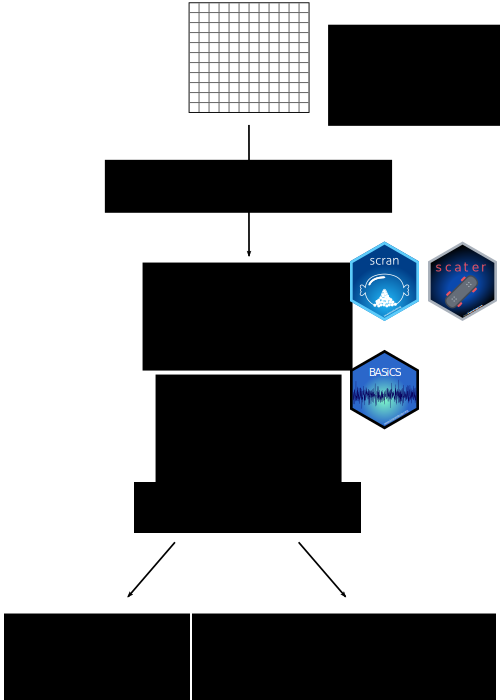
\includegraphics[width=0.5\linewidth]{figure/Overview} 

}

\caption{Graphical overview for the scRNA-seq analysis workflow described in this manuscript. Starting from a SingleCellExperiment object, we use the scater and scran Bioconductor packages to perform quality control and initial exploratory analyses. The primary focus of this workflow is to robustly quantify transcriptional heterogeneity within seemingly homogeneous cell populations. For this purpose, we apply the BASiCS Bioconductor package, illustrating how BASiCS can be used to analyse a single or multiple pre-specified groups of cells.}\label{fig:overview}
\end{figure}

\hypertarget{input-data---singlecellexperiment}{%
\subsection{\texorpdfstring{Input data - \texttt{SingleCellExperiment}}{Input data - SingleCellExperiment}}\label{input-data---singlecellexperiment}}

Here, we use the \emph{\href{https://bioconductor.org/packages/3.11/SingleCellExperiment}{SingleCellExperiment}} package to convert an input
matrix of raw read-counts (molecule counts for UMI-based protocols) into a
\texttt{SingleCellExperiment} object.
Such object can be used to store scRNA-seq data and its associated metadata,
such as gene- and cell-specific information.
Moreover, when available, the same object can be used to store read-counts for
technical spike-in molecules (these can be accessed via the \texttt{altExp()} method).
A major advantage of using a \texttt{SingleCellExperiment} object as the input for
scRNA-seq analyses is that it enables interoperability across a large number of
Bioconductor packages \citep{Amezquita2019}.

\hypertarget{quality-control-and-exploratory-analyses---scater-and-scran}{%
\subsection{\texorpdfstring{Quality control and exploratory analyses - \texttt{scater} and \texttt{scran}}{Quality control and exploratory analyses - scater and scran}}\label{quality-control-and-exploratory-analyses---scater-and-scran}}

An critical step in scRNA-seq analyses is to apply quality control (QC)
diagnostics, removing low quality samples (wells or droplets, depending on
the protocol) that may distort downstream analyses.
Among others, QC can help to identify samples that contain broken cells, that
are empty or that contain multiple cells \citep{Ilicic2016classification}.
Moreover, lowly expressed genes for which less reliable information is
available are typically also removed.
To perform QC of scRNA-seq data, we use the \emph{\href{https://bioconductor.org/packages/3.11/scater}{scater}} Bioconductor
package \citep{McCarthy2017}.
In \emph{\href{https://bioconductor.org/packages/3.11/scater}{scater}}, the \texttt{calculateQCMetrics} function can be used to
calculate standard QC metrics for each cell (e.g.~percentage of mitochondrial
reads) and gene (e.g.~percentage of zeroes across all cells).
The package also provides a suite of visualisation tools that can be used to
explore the data under study and its associated QC diagnostic metrics.

The \emph{\href{https://bioconductor.org/packages/3.11/scran}{scran}} package offers additional tools for QC
diagnostics and a variety of functions scRNA-seq data analysis \citep{Lun2016}.
In particular, it can perform \emph{global scaling} data normalisation, calculating
cell-specific scaling factors that capture global differences in read-counts
across cells (e.g.~due to variability in sequencing depth and PCR amplification)
\citep{Lun2016pooling}.
In \emph{\href{https://bioconductor.org/packages/3.11/scran}{scran}}, users can also explore how the observed variability in
gene expression counts can be decomposed into technical and biological
components (see the \texttt{decomposeVar} function).
Moreover, the \texttt{trendVar} function can be used to infer an overall trend between
gene-specific mean and variance estimates.
To derive gene-specific variability estimates that are not confounded by this
overall trend, the \texttt{DM} function calculates the distance between gene-specific
squared coefficients of variation (CV\(^2\)) and a rolling median along the range
of mean expression values \citep{Kolodziejczyk2015cell}.
DM variability estimates enable exploratory analyses of cell-to-cell
heterogeneity, but a measure of uncertainty is not readily available.
As such, gene-specific downstream inference (such as differential variability
testing) is precluded.

\hypertarget{quantifying-cell-to-cell-transcriptional-variability---basics}{%
\subsection{\texorpdfstring{Quantifying cell-to-cell transcriptional variability - \texttt{BASiCS}}{Quantifying cell-to-cell transcriptional variability - BASiCS}}\label{quantifying-cell-to-cell-transcriptional-variability---basics}}

The \emph{\href{https://bioconductor.org/packages/3.11/BASiCS}{BASiCS}} package implements a Bayesian hierarchical framework
which borrows information across all genes and cells to robustly quantify
transcriptional variability \citep{Vallejos2015BASiCS}.
Similar to the approach adopted in \emph{\href{https://bioconductor.org/packages/3.11/scran}{scran}}, \emph{\href{https://bioconductor.org/packages/3.11/BASiCS}{BASiCS}}
infers cell-specific global scaling normalisation parameters.
However, instead of inferring these as a pre-processing step,
\emph{\href{https://bioconductor.org/packages/3.11/BASiCS}{BASiCS}} uses an integrated approach in which data normalisation
and downstream analyses are performed simultaneously --- whilst propagating
statistical uncertainty.
To quantify technical noise, the original implementation of
\emph{\href{https://bioconductor.org/packages/3.11/BASiCS}{BASiCS}} uses information from extrinsic spike-in molecules as
control features, but the model has been extended to address situations in which
spike-ins are not available \citep{Eling2018}.

\emph{\href{https://bioconductor.org/packages/3.11/BASiCS}{BASiCS}} summarises the distribution of gene expression through
gene-specific \emph{mean} (\(\mu_i\)) and \emph{over-dispersion} (\(\delta_i\)) parameters.
Mean parameters \(\mu_i\) quantify the overall expression for each gene \(i\)
across the population of cells under study.
Instead, \(\delta_i\) captures the excess of variability that is observed with
respect to what would be expected in a homogeneous cell population, after
taking into account technical noise.
This is used as a proxy to quantify transcriptional variability.
Moreover, to account for the strong association that is typically observed
between mean expression and over-dispersion estimates, we recently introduced
gene-specific \emph{residual over-dispersion} parameters \(\epsilon_i\) \citep{Eling2018}.
Similar to DM values implemented in \emph{\href{https://bioconductor.org/packages/3.11/scran}{scran}}, these are defined as
deviations with respect to an overall regression trend that captures the
relationship between mean and over-dispersion values.

Parameter estimation is implemented in the \texttt{BASiCS\_MCMC} function, which can be
run using four different major settings (Table 1).
If spike-in molecules are available and \texttt{WithSpikes\ =\ TRUE} (default), the model
uses this information in order to infer technical noise.
Alternatively, if \texttt{WithSpikes\ =\ FALSE}, the approach introduced in \citep{Eling2018}
is applied.
We recommend to use \texttt{Regression\ =\ TRUE} (default) as the underlying informative
prior improves the stability of posterior estimates for small sample sizes and
lowly expressed genes \citep{Eling2018}.
Moreover, it provides additional flexibility for downstream analysis as it also
infers gene-specific residual over-dispersion parameters \(\epsilon_i\).

\begin{table}[htbp]
\caption{Four settings available for the the \texttt{BASiCS\_MCMC} function.}
\centering
\begin{tabledata}{@{}lll@{}}
\header & No regression & Regression\\
\row Using spike-in reads & \texttt{WithSpikes\ =\ TRUE} & \texttt{WithSpikes\ =\ TRUE}\\
\row & \texttt{Regression\ =\ FALSE} & \texttt{Regression\ =\ TRUE}\\
\row No spike-ins available & \texttt{WithSpikes\ =\ FALSE} & \texttt{WithSpikes\ =\ FALSE}\\
\row & \texttt{Regression\ =\ FALSE} & \texttt{Regression\ =\ TRUE}\\
\end{tabledata}
\end{table}

The algorithm implemented in the \texttt{BASiCS\_MCMC} function is an adaptive
Metropolis within Gibbs sampler \citep{Roberts2009}.
The \texttt{BASiCS\_MCMC} function returns a \texttt{BASiCS\_Chain} object, which can be used
for further downstream analyses, many of which are detailed in this workflow.
These objects contain draws from Markov chain Monte Carlo (MCMC) samplers,
which are used to infer the posterior distribution over the model parameters
\citep{Smith1993}.
Briefly, the posterior distribution quantifies how probable different parameter
values are given the observed data. However, before assessing the posterior
distribution, we must first ensure that the MCMC sampler has converged to
its stationary distribution, and has sampled efficiently from this distribution
\citep{Cowles1996}. If these conditions are not met, then the estimated parameters
may be inaccurate. The \emph{\href{https://CRAN.R-project.org/package=coda}{coda}} CRAN package contains a variety of
functions to assess the convergence of a sampled MCMC chain.
To use \texttt{coda} functions, the individual chains returned by \texttt{BASiCS} need to be
transformed into a MCMC object that \texttt{coda} recognises using the \texttt{coda::mcmc}
function. \texttt{BASiCS} also offers a number of functions to visualise and assess the
convergence of MCMC chains. In particular, we will use
\texttt{BASiCS\_EffectiveSize} and \texttt{BASiCS\_DiagPlot} to calculate and visualise the
effective sample size generated by the MCMC samplers.

{[}talk about downstream analyses; hvg/lvg; differential testing
then mention the ability to perform differential testing;
finally the extention to account for mean/over-dispersion{]}

{\small\bibliography{Workflow.bib}}

\end{document}
